\documentclass{report}
\usepackage[utf8]{inputenc}
\usepackage{booktabs}
\usepackage{graphicx}
\usepackage[italian]{babel}
\usepackage{hyperref}
\usepackage[T1]{fontenc}
\usepackage[utf8]{inputenc}
\usepackage[italian]{babel}
\usepackage{eucal,enumitem}
\usepackage{longtable}
\usepackage{amsmath,amssymb,amsthm}
\usepackage{tikz}
\usepackage{cancel} 
\usepackage{multirow}
\usepackage{multicol}
\usepackage{color}
\usepackage{tabto}
\usepackage{fancyhdr}
\usepackage{xltabular}
\usepackage{pdfpages}

\begin{document}
    \begin{figure}[htbp!]
        \begin{center}
            
\includegraphics[width=.25\textwidth]{Immagini/FedericoII.png}
        \end{center}
    \end{figure}
\begin{center}
    {\scshape\Large\bfseries\center  Progetto Di Basi Di Dati 2022/2023 \\ Sistema Di Gestione Di Personale E Progetti All’Interno Di Un’Azienda }
\end{center}
\vfill
    \begin{center}
	Napolano\tab								Liberti	\\
	Emilia\tab									Simone	\\
	N86004758\tab								N86004252 \\
		\begin{center}
			  Novembre 2022
		\end{center}			
    \end{center}
    \newpage
    
    \tableofcontents
    
    \chapter{Analisi del progetto e requisiti individuati}
\section{Dipendenti dell'azienda}
Per ogni dipendente si assegnerà una categoria basata sul numero di anni di servizio. Ogni dipendente appartiene a una sola fra quattro categorie:
\begin{itemize}
    \item Dipendente Junior
    \item Dipendente Middle
    \item Dipendente Senior
    \item Dipendente Dirigente
\end{itemize}
Ogni dipendente può essere identificato con un nome, un cognome e un identificativo unico nel sistema (codice fiscale). Per ogni dipendente può essere specificato una mansione e un ufficio.

\section{Passaggio di ruolo}
Le categorie sono assegnate ai dipendenti in base all'anzianità, rispettivamente:
\begin{itemize}
    \item Junior: meno di 3 anni
    \item Middle: compreso tra 3 e 7 anni
    \item Senior: più di 7 anni
\end{itemize}
L'unica categoria che non richiede anzianità è la categoria Dirigente, che può essere raggiunta solo in base alle proprie capacità.
Di conseguenza sarà necessario tracciare i dati di carriera di ogni dipendente, memorizzando la prima data di assunzione e il numero di anni di servizio attraverso un'entità separata. 

\section{Gestione dei laboratori}
I laboratori sono formati da gruppi di dipendenti di qualsiasi categoria che lavorano a specifici topic di un determinato progetto. Un laboratorio può essere gestito solo da un dipendente senior, che avrà titolo di responsabile scientifico. Ad ogni progetto saranno assegnati al più 3 laboratori.

\section{Gestione dei progetti}
Un progetto è identificato da un CUP (Codice Unico Progetto) e da un nome (unico nel sistema). Ogni progetto può essere gestito solo da un dipendente Dirigente e avrà, come per i laboratori, un referente scientifico, che potrà essere solo un dipendente senior.

\section{Requisiti aggiuntivi}
Come requisiti aggiuntivi sono stati identificati:
\begin{itemize}
    \item Tracciamento dei contratti
    \item Collaborazione tra più aziende
\end{itemize}
Un contratto può essere caratterizzato da un tipo e una durata temporale, oltre a tenere traccia della data della firma e del salario. \\
Più aziende possono collaborare a uno stesso progetto. \\
Un contratto a tempo determinato viene rinnovato automaticamente ogni 3 anni.
Un dipendente puo' avere un aumento di salario anche senza passaggio di ruolo o senza aver firmato un nuovo contratto.
    \chapter{Progettazione concettuale}
\section{Introduzione}
In questa sezione verrà introdotta la progettazione concettuale dell'applicativo. Partendo da un primo diagramma di classe in UML. Dal risultato dell'analisi dei requisiti che devono essere soddisfatti si arriverà a uno schema concettuale ristrutturato. Saranno evidenziati i concetti rilevanti ai fini della rappresentazione dei dati e le relazioni che intercorrono tra di esse.

\section{Class Diagram}
\begin{figure}[!h]
    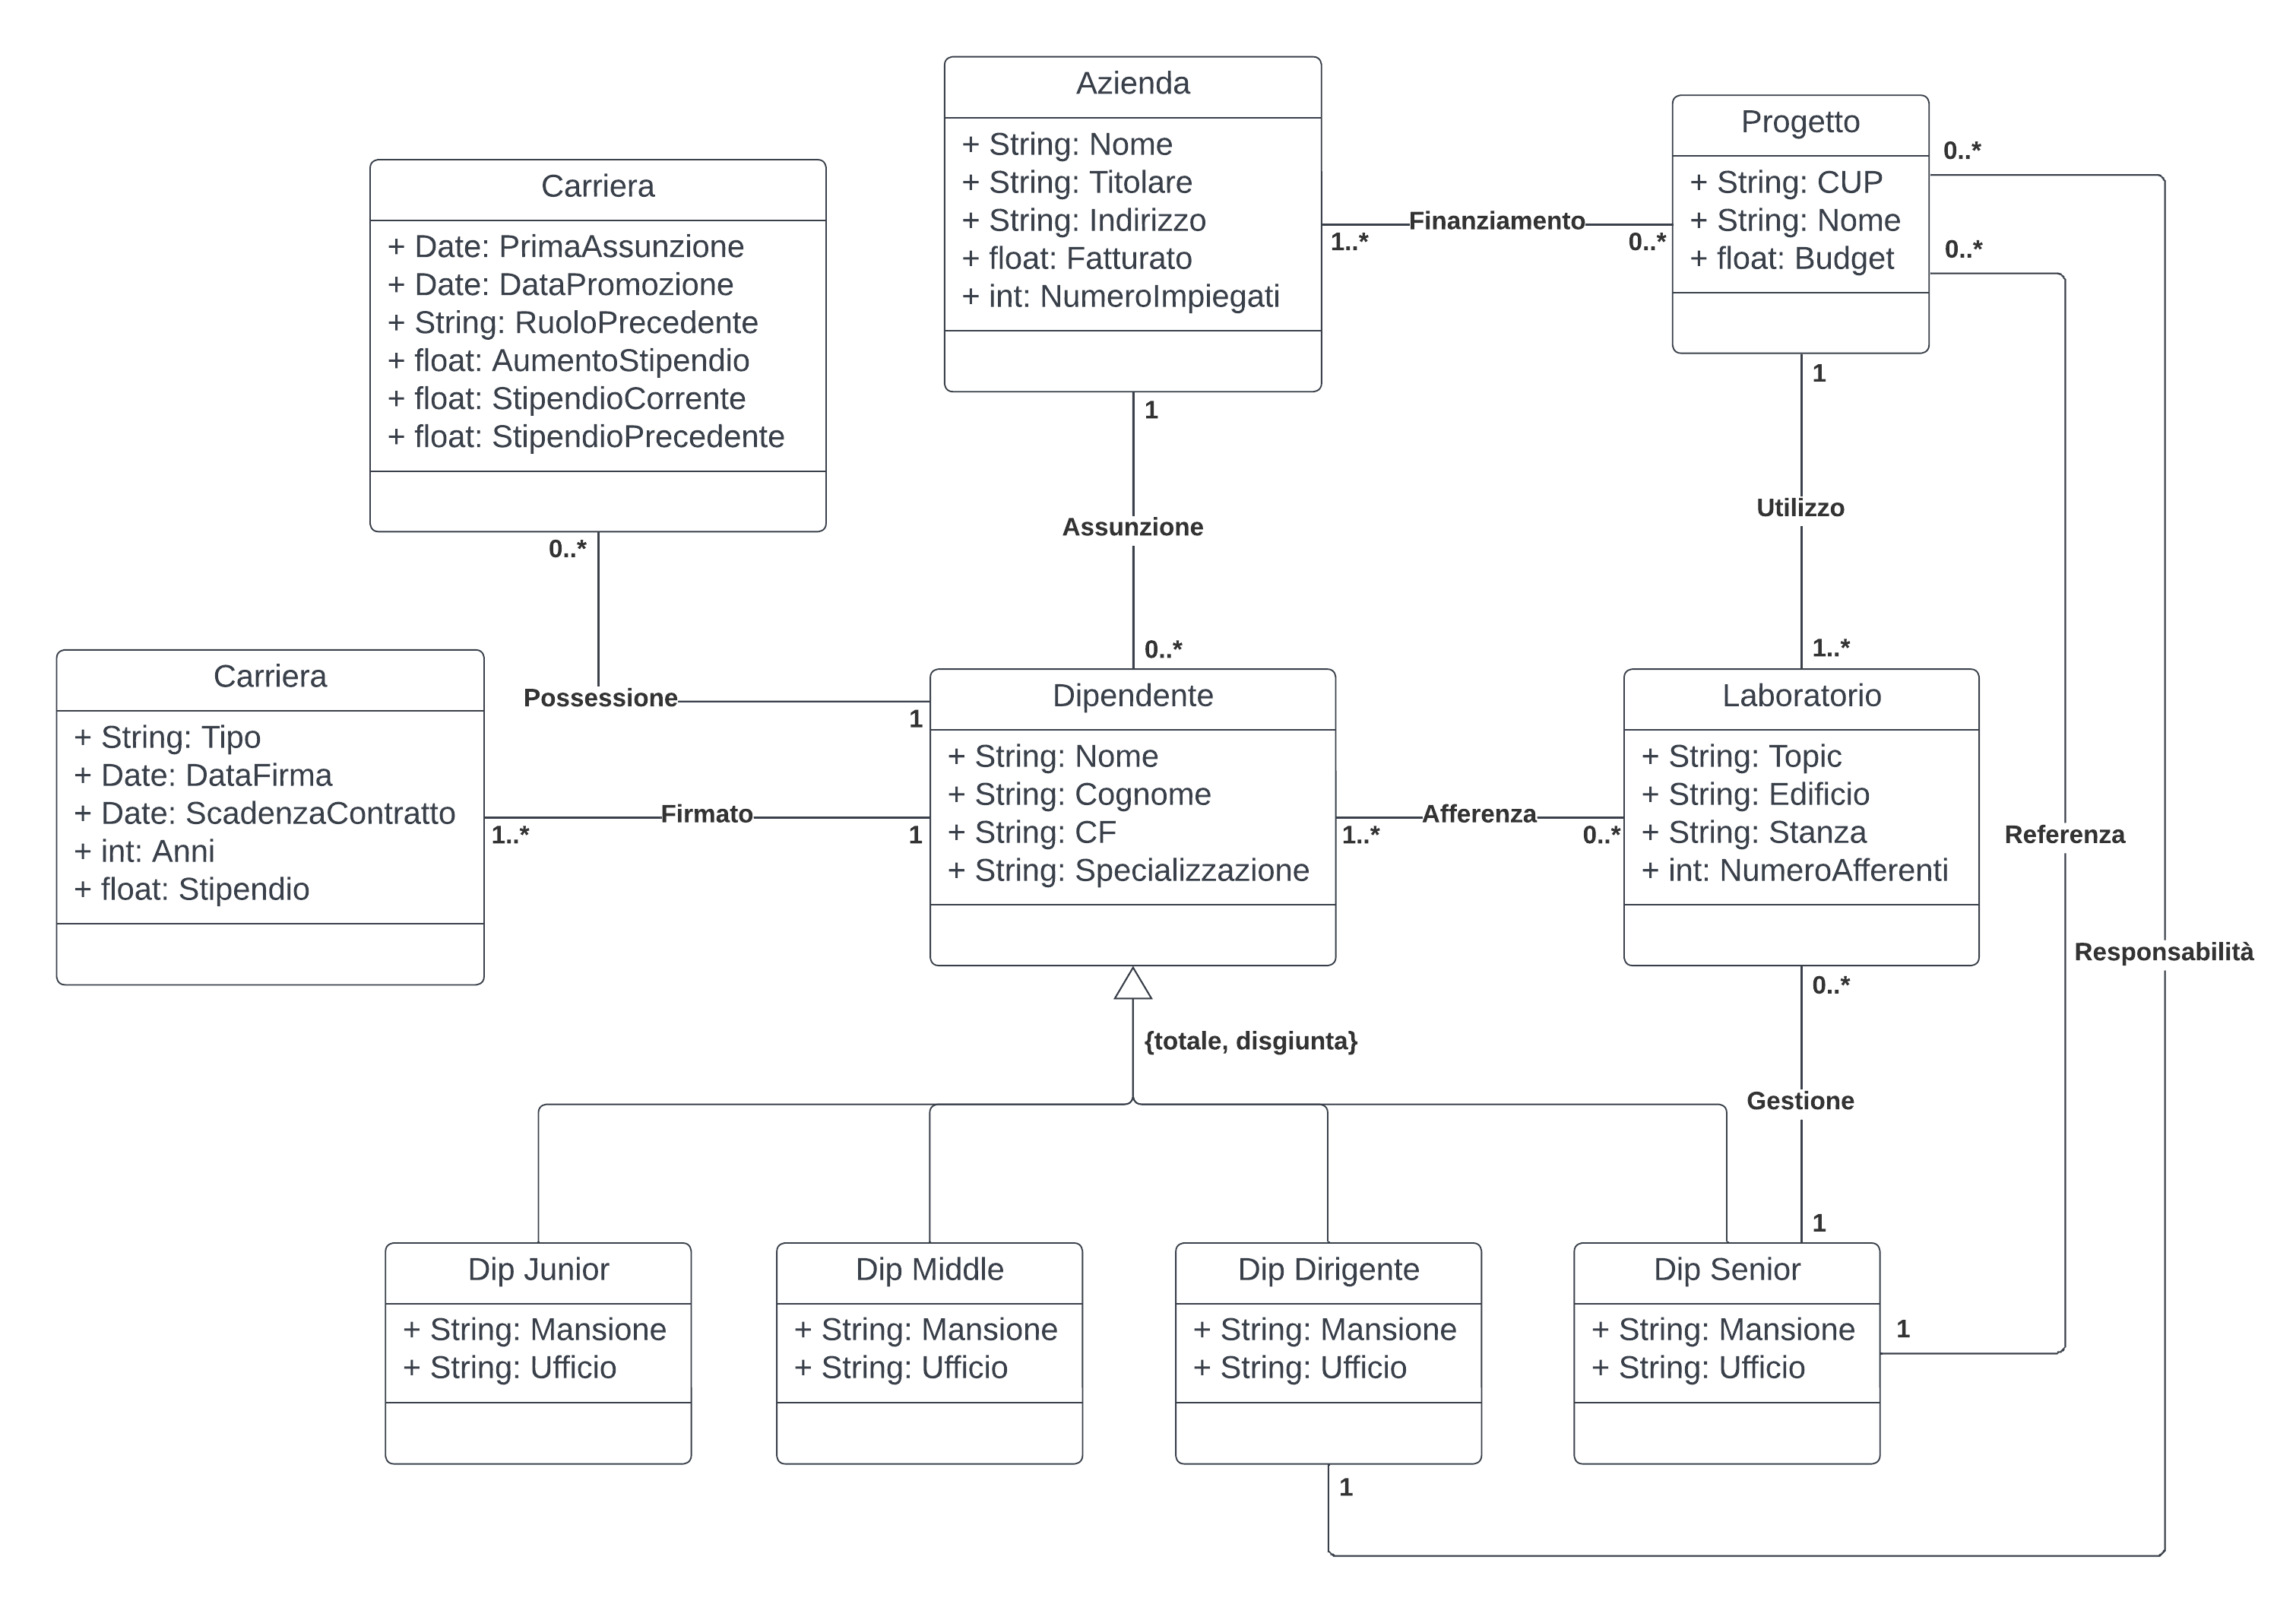
\includegraphics[width=.8\linewidth]{./Immagini/BozzaProgetto.png}
\end{figure}

\section{Ristrutturazione del Class Diagram}
Al fine di rendere il class diagram idoneo alla traduzione logica e di migliorare l’efficienza dell’implementazione si procede alla ristrutturazione dello stesso.

\subsection{Analisi delle ridondanze}
Sono ora anlizzate le ridondanze trovate all'interno del Class Diagram precedente:
\begin{itemize}
    \item Il numero degli impiegati può essere ricavato attraverso la relazione assunzione,
    \item Il numero di anni di contratto può essere ricavato sottraendo alla data di scadenza la data di assunzione,
    \item Il numero di afferenti di un laboratorio può essere ricavato contando i dipendenti dalla relazione Afferenza.
\end{itemize}
Da ricordare che la rimozione delle ridondanze è specifica alla progettazione concettuale: in fase di implementazione potrebbe rivelarsi conveniente introdurre alcuni attributi ridondanti al fine di facilitare le query (un esempio sono StipendioPrecedente e StipendioCorrente).

\subsection{Analisi degli identificativi}
Per facilitare la traduzione verso lo schema logico e per il recupero efficiente dei dati si inseriscono gli identificativi IDContratto e IDCarriera, rispettivamente alle entità Contratto e Carriera.
Per identificare univocamente i dipendenti sarà considerato unico il codice fiscale. Per l'azienda sono presi come identificativi il nome e la via, mentre per il progetto sarà utilizzato il CUP. Infine per il laboratorio si possono considerare univoci nel sistema tutti i suoi attributi, ovvero "Topic, Edificio, Stanza".


\subsection{Rimozione degli attributi multivalore}
Il nome e il cognome del titolare dell'azienda saranno considerati come una stringa unica.

\subsection{Rimozione degli attributi composti}
Nell'entità Azienda l'attributo Indirizzo sarà estratto in modo da delineare gli attributi: "Via, Civico, CAP".

\subsection{Partizione/Accorpamento delle associazioni}
Non vengono eseguiti accorpamenti o partizioni delle associazioni.

\subsection{Rimozione delle gerarchie}
La disgiunzione totale tra la superclasse Dipendente e le sottoclassi Dipendente Junior, Dipendente Middle, Dipendente Senior e Dipendente Dirigente viene eliminata accorpando le sottoclassi nella superclasse: sarà necessario inserire un attributo "Ruolo" per controllare la categoria del dipendente.\\
Sarà anche necessario modificare le molteplicità delle associazioni tra la classe Dipendente e le classi Progetto e Laboratorio.
\newpage
\section{Diagrammi ristrutturati}
\subsection{Class Diagram}
\begin{figure}[!h]
    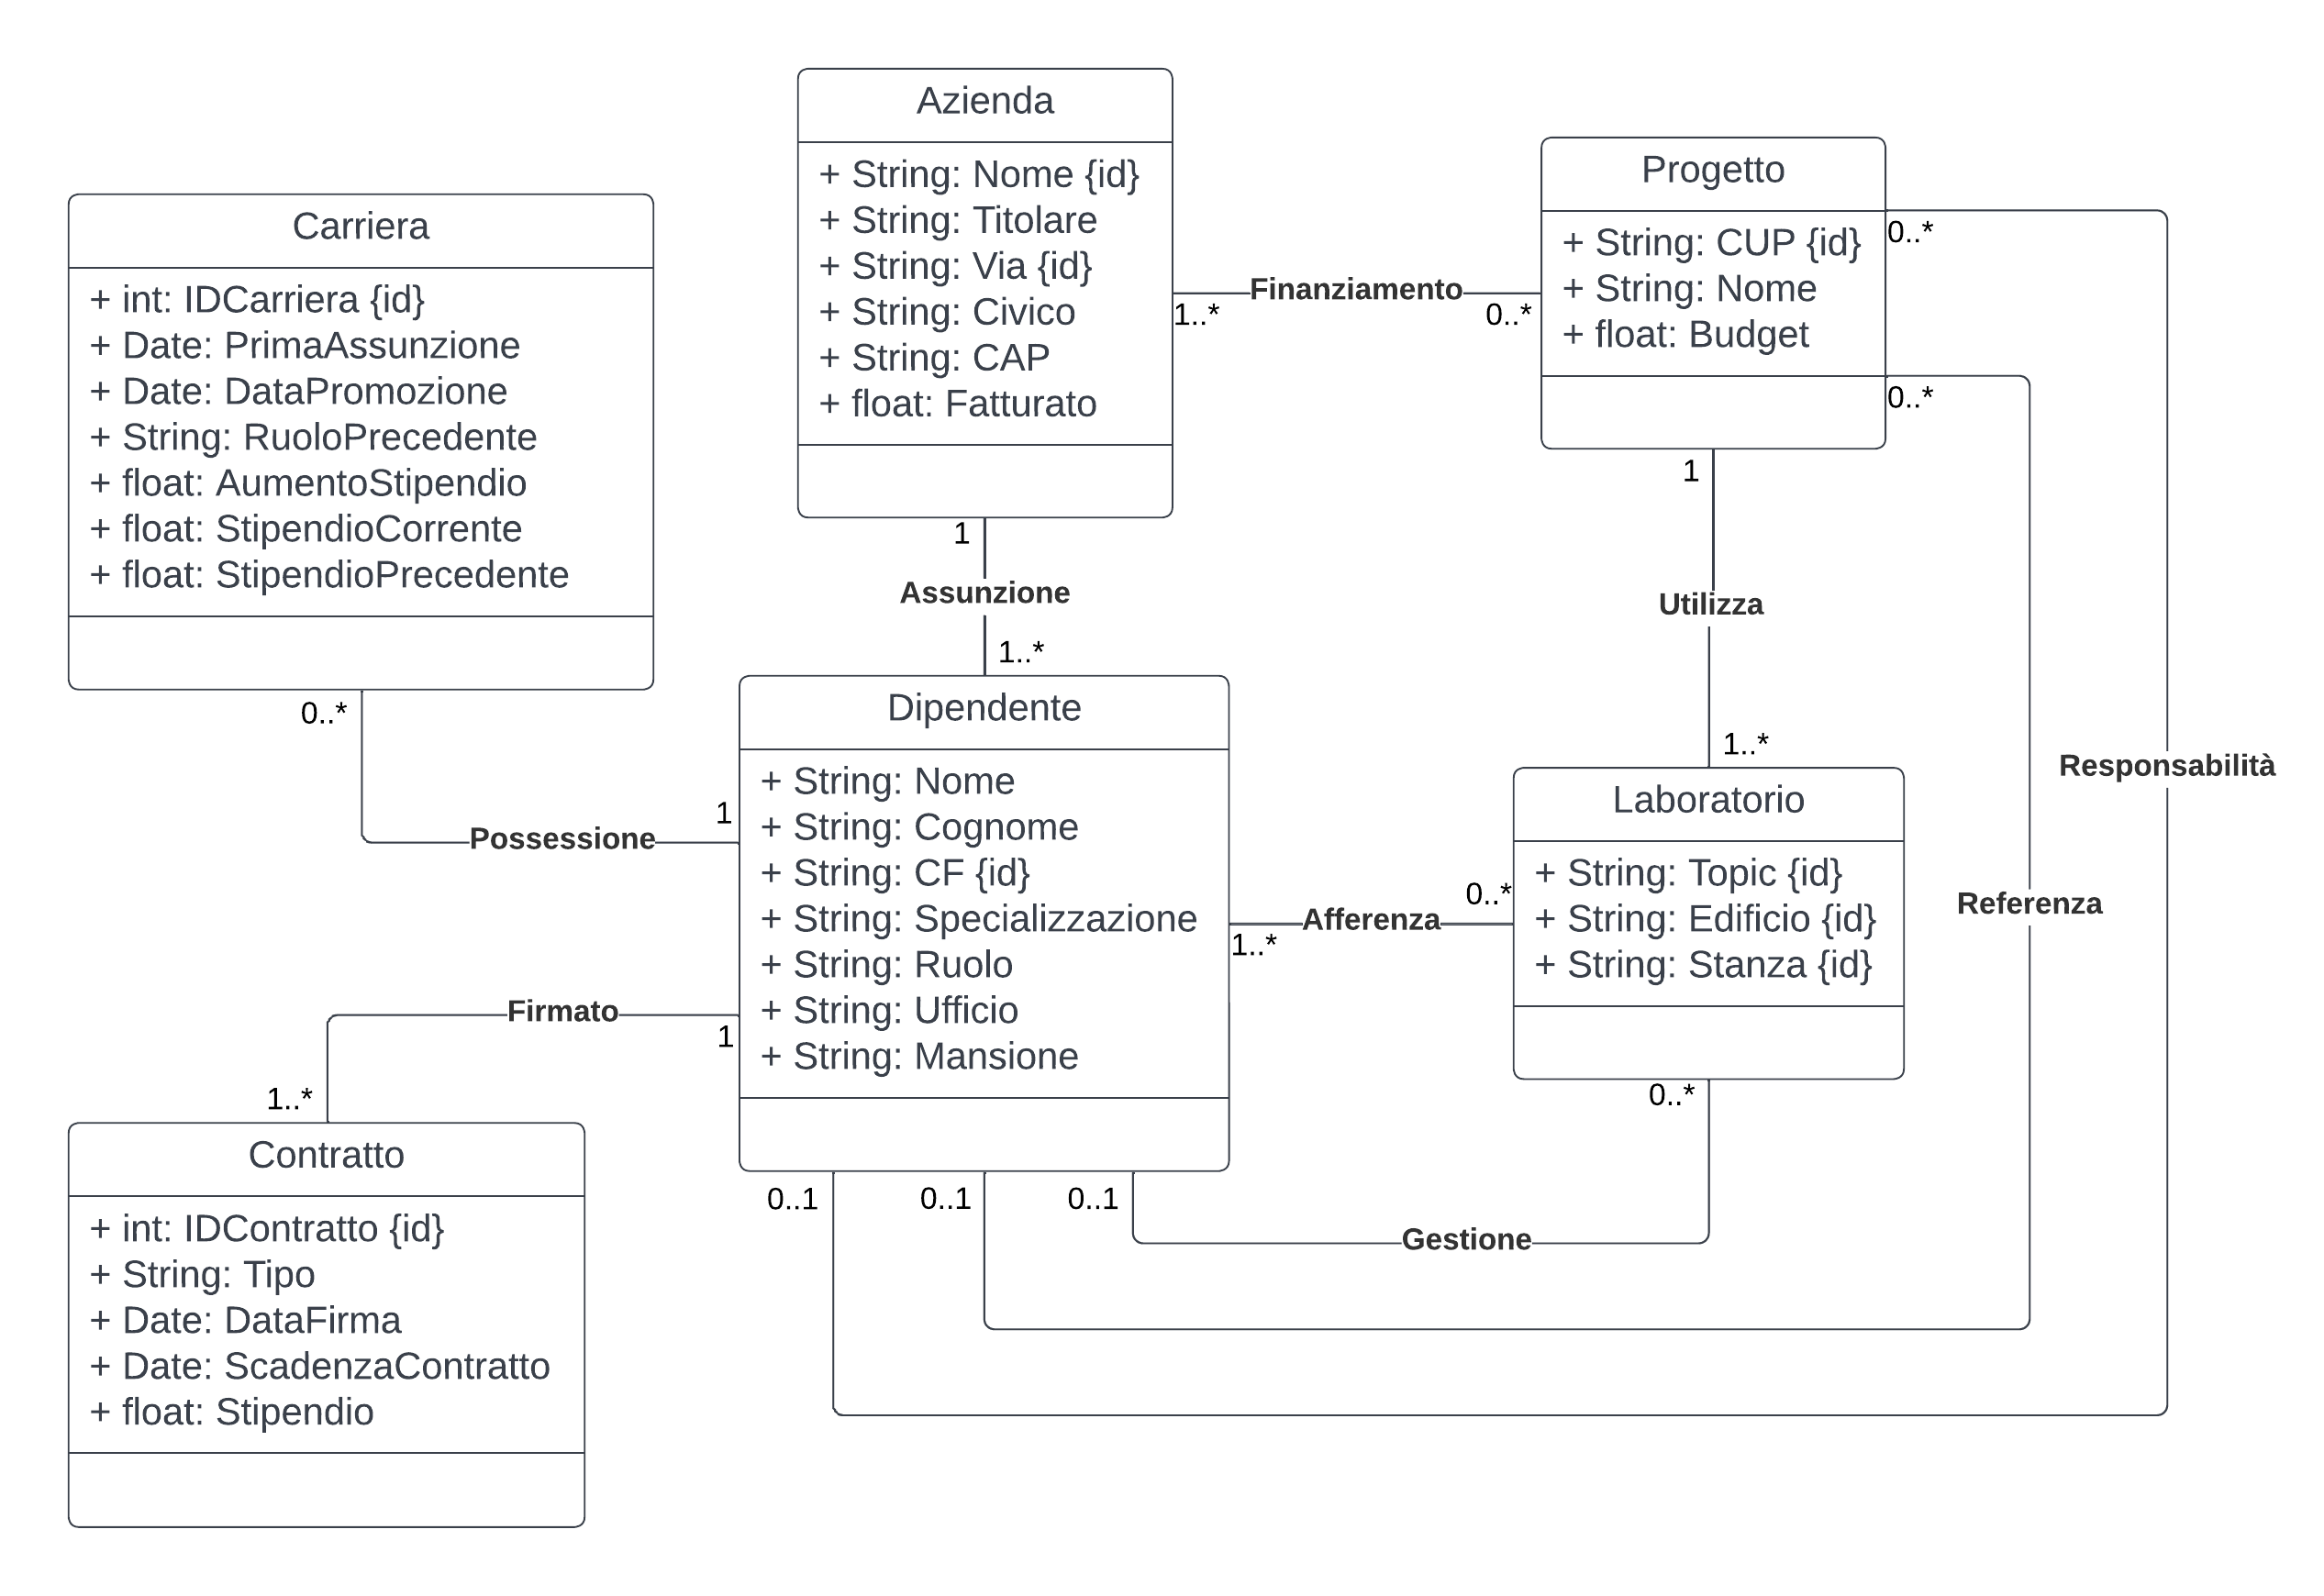
\includegraphics[width=.8\linewidth]{./Immagini/Ristrutturato.png}
\end{figure}
\subsection{Diagramma ER}
\begin{figure}[!h]
    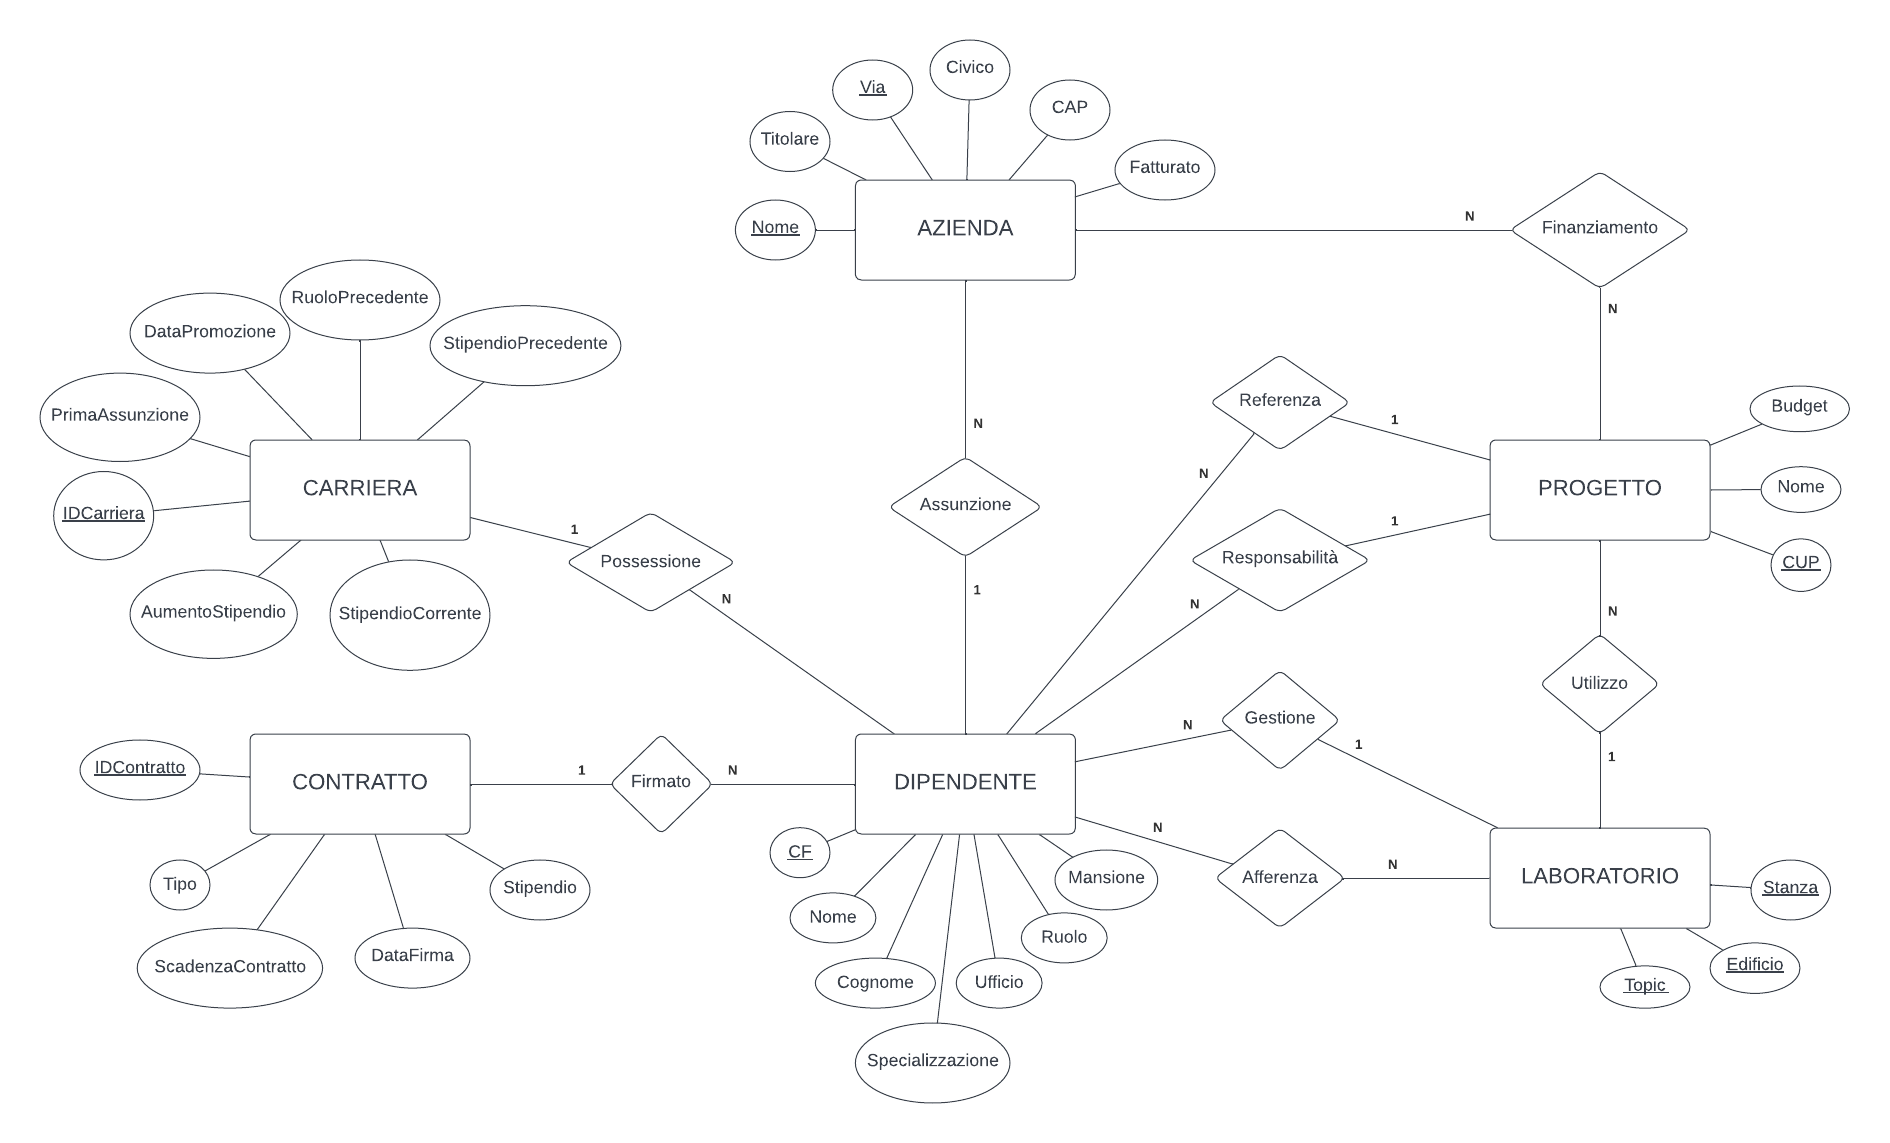
\includegraphics[width=.8\linewidth]{./Immagini/ER.png}
\end{figure}
    \chapter{Dizionari}
\section{Introduzione}
In questo capitolo verranno analizzate le singole entità, le loro associazioni ed eventuali vincoli e di seguito riportato un dizionario contenente le loro descrizioni e caratteristiche. 

\section{Dizionario delle classi}

\begingroup
    \setlength{\tabcolsep}{6pt}
    \renewcommand{\arraystretch}{1.5}
    \begin{xltabular}{\textwidth}{l X X}
        \caption{Dizionario delle classi.} \label{tab:classi} \\

        \hline \multicolumn{1}{|l}{\textbf{Classe}} & \multicolumn{1}{X}{\textbf{Descrizione}} & \multicolumn{1}{X|}{\textbf{Attributi}} \\ \hline 
        \endfirsthead

        \multicolumn{3}{c}%
        {\tablename\ \thetable{} Dizionario delle classi} \\
        \hline \multicolumn{1}{|l}{\textbf{Classe}} & \multicolumn{1}{X}{\textbf{Descrizione}} & \multicolumn{1}{X|}{\textbf{Attributi}} \\ \hline 
        \endhead

        \multicolumn{3}{r}{{Continua nella pagina successiva}} \\ 
        \hline
        \endfoot

        \hline
        \endlastfoot

        \textbf{Azienda} & Entità descrittrice di un tipo generico di Azienda & \textbf{Nome} (String): Nome dell'azienda, identifica univocamente un'azienda.
        \newline\textbf{Titolare} (String): Nome del titolare dell'azienda.
        \newline\textbf{Via} (String): Via della sede dell'azienda, identifica univocamente un'azienda.
        \newline\textbf{Civico} (String): Civico della sede dell'azienda.
        \newline\textbf{CAP} (String): Codice di avviamento postale.
        \newline\textbf{Fatturato} (float): Fatturato dell'azienda.\\
        \hline

        \textbf{Dipendente} & Entità descrittrice di un profilo generico di un dipendente aziendale & \textbf{Nome} (String): Nome del dipendente.
        \newline\textbf{Cognome} (String): Cognome del dipendente.
        \newline\textbf{CF} (String): Codice Fiscale del dipendente, identifica univocamente un dipendente.
        \newline\textbf{Specializzazione} (String): Laurea del dipendente (se conseguita).
        \newline\textbf{Ruolo} (String): Categoria di appartenenza del dipendente.
        \newline\textbf{Ufficio} (String): Ufficio dove lavora il dipendente.
        \newline\textbf{Mansione} (String): Lavoro svolto abitualmente dal dipendente. \\
        \hline

        \textbf{Contratto} & Entità descrittrice di un contratto firmato da un dipendente per una certa azienda & \textbf{IDContratto} (int): identifica univocamente un contratto.
        \newline\textbf{Tipo} (String): Tipo di contratto firmato.
        \newline\textbf{DataFirma} (Date): Data in cui il dipendente firma il contratto.
        \newline\textbf{ScadenzaContratto} (Date): Data in cui scade il contratto (se è a tempo determinato).
        \newline\textbf{Stipendio} (float): Stipendio accordato al momento della firma del contratto.\\
        \hline
        \textbf{Carriera} & Entità descrittrice della carriera attuale o pregressa di un dipendente. &  \textbf{IDCarriera} (int): identifica univocamente una carriera
        \newline\textbf{PrimaAssunzione} (Date): Data di prima assunzione del dipendente.
        \newline\textbf{DataPromozione} (Date): Data della promozione del dipendente.
        \newline\textbf{RuoloPrecedente} (String): Ultimo ruolo ricoperto dal dipendente prima della promozione.
        \newline\textbf{AumentoStipendio} (float): Aumento stipendio in percentuale.
        \newline\textbf{StipendioCorrente} (float): Stipendio aumentato a seguito dell'aumento di stipendio. 
        \newline\textbf{StipendioPrecedente} (float): Stipendio prima dell'aumento. \\
        \hline

        \textbf{Progetto} & Entità descrittrice di un progetto finanziato da un'azienda & \textbf{CUP} (String): Codice Unico Progetto, identifica univocamente un progetto. 
        \newline\textbf{Nome} (String): Nome del progetto. 
        \newline\textbf{Budget} (float): Budget del progetto. \\
        \hline

        \textbf{Laboratorio} & Entità descrittrice di un laboratorio. & \textbf{Topic} (String): Argomento principale del laboratorio, identifica univocamente un laboratorio.
        \newline\textbf{Edificio} (String): Edificio in cui è situato il laboratorio, identifica univocamente un laboratorio. 
        \newline\textbf{Stanza} (String): Stanza in cui è situato il laboratorio, identifica univocamente un laboratorio. \\

    \end{xltabular}
\endgroup

\newpage
\section{Dizionario delle associazioni}

\begingroup
    \setlength{\tabcolsep}{6pt}
    \renewcommand{\arraystretch}{2.0}
    \begin{xltabular}{\textwidth}{l X X}
        \caption{Dizionario delle associazioni.} \label{tab:associazioni} \\
        
        \hline \multicolumn{1}{|l}{\textbf{Nome}} & \multicolumn{1}{X}{\textbf{Descrizione}} & \multicolumn{1}{X|}{\textbf{Classi coinvolte}} \\ \hline 
        \endfirsthead
        
        \multicolumn{3}{c}%
        {\tablename\ \thetable{} Dizionario delle associazioni} \\
        \hline \multicolumn{1}{|l}{\textbf{Nome}} & \multicolumn{1}{X}{\textbf{Descrizione}} & \multicolumn{1}{X|}{\textbf{Classi coinvolte}} \\ \hline 
        \endhead
        
        \multicolumn{3}{r}{{Continua nella pagina successiva}} \\ 
        \hline
        \endfoot
        
        \hline
        \endlastfoot

        \textbf{Finanziamento} & Esprime la relazione tra l'azienda e il progetto. Un'azienda finanzia uno o più progetti, un progetto è finanziato da una o più aziende. & \textbf{Azienda [1...*]} ruolo \textbf{finanzia:} indica la/le aziende che finanziano un progetto. 
        \newline\textbf{Progetto [0...*]} ruolo \textbf{è finanziato da:} indica progetti che sono finaziati da una o più aziende. \\
        \hline
        \textbf{Assunzione} & Esprime la relazione tra l'azienda e il dipendente. Un'azienda assume uno o più dipendenti, un dipendente è assunto da un'azienda. & \textbf{Azienda [1]} ruolo \textbf{assume:} indica l'azienda che assume un dipendente. 
        \newline\textbf{Dipendente [1...*]} ruolo \textbf{è assunto da:} indica dipendenti che sono assunti da un'azienda. \\
        \hline
        \textbf{Possessione} & Esprime la relazione tra dipendente e carriera. Un dipendente possiede una o più carriere, una carriera è posseduta da un solo dipendente. & \textbf{Dipendente [1]} ruolo \textbf{possiede:} indica il dipendente che possiede una carriera. 
        \newline\textbf{Carriera[0...*]} ruolo \textbf{è posseduta da:} indica la carriera attuale o le carriere pregresse possedute da un dipendente. \\
        \hline
        \textbf{Firmato} & Esprime la relazione tra dipendente e contratto. Un dipendente firma uno o più contratti, un contratto è firmato da un solo dipendente. & \textbf{Dipendente [1]} ruolo \textbf{firma:} indica il dipendente che firma un contratto. 
        \newline\textbf{Contratto [1...*]} ruolo \textbf{è firmato da:} indica il/i contratti firmati da un dipendente.\\
        \hline
        \textbf{Gestione} & Esprime la relazione tra dipendente senior e laboratorio. Un dipendente gestisce più laboratori, un laboratorio è gestito da un solo dipendente. & \textbf{Dipendente [0...1]} ruolo \textbf{gestisce:} indica il dipendente che gestisce un laboratorio. 
        \newline\textbf{Laboatorio [0...*]} ruolo \textbf{è gestito da:} indica il laboratorio che è gestito da un dipendente. \\
        \hline
        \textbf{Referenza} & Esprime la relazione tra dipendente senior e progetto. Un dipendente è referente di uno o più progetti, un progetto è referenziato da un solo dipendente. & \textbf{Dipendente [0...1]} ruolo \textbf{è referente di:} indica il dipendente che è referente scientifico di un progetto. 
        \newline\textbf{Progetto [0...*]} ruolo \textbf{è referenziato da:} indica il progetto che è referenziato da un dipendente.\\
        \hline
        \textbf{Responsabilità} & Esprime la relazione tra dirigente e progetto. Un dipendente è responsabile di uno o più progetti, un progetto ha come responsabile un solo dipendente. & \textbf{Dipendente [0...1]} ruolo \textbf{è responsabile di:} indica il dipendente che è responsabile di un progetto. 
        \newline\textbf{Progetto [0...*]} ruolo \textbf{ha come responsabile:} indica il progetto che ha come responsabile un dipendente.\\
        \hline
        \textbf{Afferenza} & Esprime la relazione tra dipendente e laboratorio. Un dipendente afferisce a uno o più laboratori, un laboratorio è afferito da uno o più dipendenti. & \textbf{Dipendente [1...*]} ruolo \textbf{afferisce:} indica il dipendente che afferisce a un laboratorio. \newline\textbf{Laboratorio [0...*]} ruolo \textbf{è afferito da:} indica il laboratorio che è afferito da un dipendente. \\
        \hline
        \textbf{Utilizzo} & Esprime la relazione tra progetto e laboratorio. Un laboratorio è utilizzato da un solo progetto, un progetto utilizza uno o più laboatori. & \textbf{Laboratorio [1...*]} ruolo \textbf{è utilizzato da:} indica il laboratorio che è utilizzato da un progetto. \newline\textbf{Progetto [1]} ruolo \textbf{utilizza:} indica il progetto che utilizza un laboratorio. \\

    \end{xltabular}
\endgroup

\newpage
\section{Dizionario dei vincoli}

\begingroup
    \setlength{\tabcolsep}{6pt}
    \renewcommand{\arraystretch}{2.0}
    \begin{xltabular}{\textwidth}{l X}
        \caption{Dizionario dei vincoli.} \label{tab:vincoli} \\
        
        \hline \multicolumn{1}{|l}{\textbf{Nome Vincolo}} & \multicolumn{1}{X|}{\textbf{Descrizione}} \\ \hline 
        \endfirsthead
        
        \multicolumn{2}{c}%
        {\tablename\ \thetable{} Dizionario dei vincoli} \\
        \hline \multicolumn{1}{|l}{\textbf{Nome Vincolo}} & \multicolumn{1}{X|}{\textbf{Descrizione}} \\ \hline 
        \endhead
        
        \multicolumn{2}{r}{{Continua nella pagina successiva}} \\ 
        \hline
        \endfoot
        
        \hline
        \endlastfoot

        \textbf{Validità Nome Azienda} & Il nome di un'azienda deve essere composto unicamente da caratteri alfanumerici. \\

        \textbf{Validità Nome Titolare} & Il nome di un titolare deve essere composto unicamente da lettere. \\

        \textbf{Dominio ruoli} & Il ruolo di un dipendente può esclusivamente essere uno solo tra "Junior", "Middle", "Senior", "Dirigente". \\

        \textbf{Anzianità} & Il passaggio di ruolo da "Junior" a "Middle" deve avvenire solo dopo 3 anni di esperienza. \newline Il passaggio da "Middle" a "Senior" deve avvenire dopo 7 anni di servizio. \\

        \textbf{Gestione Laboratorio} & Un laboratorio può essere gestito solo da un dipendente "Senior". \\

        \textbf{Utilizzo Laboratori} & Un progetto può utilizzare al più 3 laboratori. \\

        \textbf{Nome Progetto} & Il nome di ogni progetto deve essere unico nel sistema. \\

        \textbf{Referenza Progetti} & Un progetto può avere come referente solo un dipendente "Senior". \\

        \textbf{Responsabilità Progetti} & Un progetto può avere come responsabile solo un dipendente "Dirigente". \\

        \textbf{Validità CF} & Un Codice Fiscale deve contenere al massimo 16 caratteri alfanumerici. \\
\hline
        \textbf{Validità Data Contratto} & La data di scadenza di un contratto non può essere precedente alla data di firma. \\

        \textbf{Validità Data Carriera} & La data di promozione di un dipendente non può essere precedente alla data di prima assunzione. \\

        \textbf{Consistenza Prima Assunzione} & La data di prima assunzione deve coincidere con la data di firma del primo contratto. \\

        \textbf{Dominio Aumento Stipendio} & Il valore di aumento di stipendio deve essere compreso tra 0 e 1 \\

        \textbf{Validità Nome e Cognome} & Il nome e cognome di ogni dipendente devono contenere almeno un carattere e solo caratteri compresi tra A-Z o a-z. \\

        \textbf{Indeterminato senza scadenza} &Se il contratto di un dipendente è a tempo indeterminato allora la scadenza del contratto deve essere null. \\
    \end{xltabular}
\endgroup
    \chapter{Progettazione Logica}
In questo capitolo verrà trattato il passaggio dalla progettazione concettuale alla progettazione logica. Nello schema che seguirà le chiavi primarie saranno identificate con una \underline{sottolineatura} e le chiavi esterne con un *.

\section{Schema Logico}

\begingroup
    \setlength{\tabcolsep}{20pt}
    \renewcommand{\arraystretch}{2.0}
    \begin{xltabular}{\textwidth}{l X}

        \textbf{Contratto} & (\underline{IDContratto}, Tipo, DataFirma, ScadenzaContratto, Stipendio, CF*)
        \newline CF $\rightarrow$ Dipendente.CF \\

        \textbf{Dipendente} & (Nome, Cognome, \underline{CF}, Specializzazione, Ruolo, Ufficio, Mansione) \\
       
        \textbf{Laboratorio} & (\underline{Topic},\underline{Edificio}, \underline{Stanza}) \\
       
        \textbf{Progetto} & (\underline{CUP}, Nome, Budget) 
        \\
        \textbf{Utilizzo} & (CUP*,Topic*,Edificio*,Stanza*)
        \newline CUP$\rightarrow$Progetto.CUP
        \newline (Topic,Edificio,Stanza)$\rightarrow$Laboratorio.(Topic,Edificio,Stanza) \\
        \textbf{Carriera} & (\underline{IDCarriera}, PrimaAssunzione, DataPromozione, RuoloPrecedente, AumentoStipendio, StipendioCorrente, StipendioPrecedente) \\

        \textbf{Possessione} & (IDCarriera*, CF*) 
        \newline IDCarriera$\rightarrow$Carriera.IDCarriera
        \newline CF $\rightarrow$ Dipendente.CF \\ 

        \textbf{Azienda} & (\underline{Nome}, Titolare,\underline{Via}, Civico, CAP, Fatturato) \\

        \textbf{Assunzione} & (Nome*, Via*, CF*) 
        \newline Nome $\rightarrow$ Azienda.Nome
        \newline Via $\rightarrow$ Azienda.Via 
        \newline CF $\rightarrow$ Dipendente.CF \\

        \textbf{Finanziamento} & (Nome*, Via*,CUP*) 
        \newline Nome $\rightarrow$ Azienda.Nome 
        \newline Via $\rightarrow$ Azienda.Via 
        \newline CUP $\rightarrow$ Progetto.CUP \\

        \textbf{Afferenza} & (CF*, Topic*, Edificio*, Stanza*) 
        \newline CF $\rightarrow$ Dipendente.CF 
        \newline (Topic,Edificio,Stanza) $\rightarrow$ Laboratorio.(Topic,Edificio,Stanza)\\
        
        \textbf{Responsabilità} & (CF*, CUP*)
        \newline CF $\rightarrow$ Dipendente.CF 
        \newline CUP $\rightarrow$ Progetto.CUP \\
        
        \textbf{Gestione} & (CF*, Topic*, Edificio*, Stanza*) 
        \newline CF $\rightarrow$ Dipendente.CF 
        \newline (Topic,Edificio,Stanza) $\rightarrow$ Laboratorio.(Topic,Edificio,Stanza) \\
        
        \textbf{Referenza} & (CF*, CUP*)
        \newline CF $\rightarrow$ Dipendente.CF 
        \newline CUP $\rightarrow$ Progetto.CUP \\

    \end{xltabular}
\endgroup

\section{Trigger e Procedure}
\subsection{Indeterminato senza scadenza}
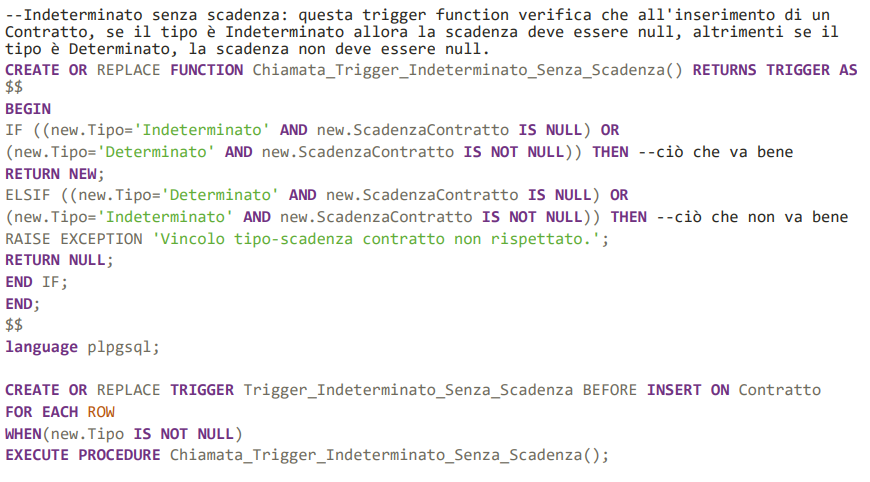
\includegraphics[width=1.2\textwidth]{Immagini/vincolo1.sql}
Esempio di cosa accade se si prova ad inserire un contratto non valido:
\newline\newline
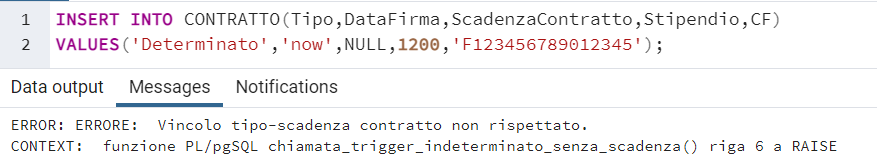
\includegraphics[width=1.2\textwidth]{Immagini/vincolo1}

\subsection{Passaggio a indeterminato}
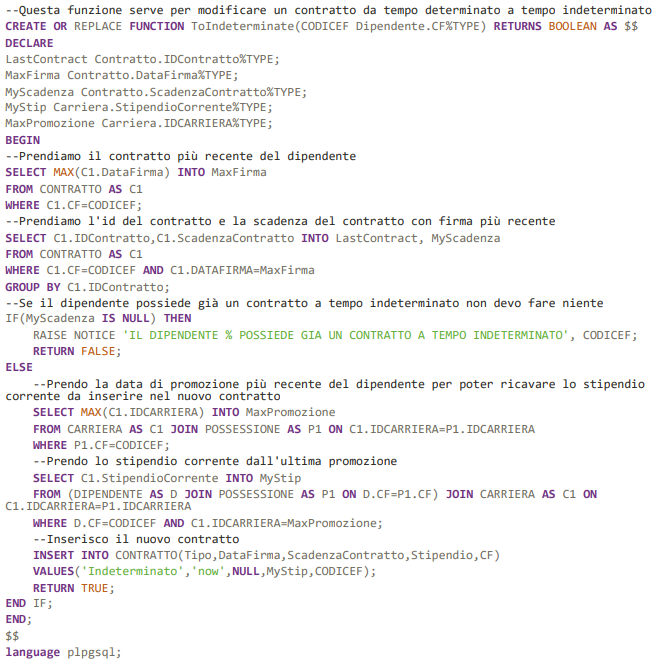
\includegraphics[width=1.2\textwidth]{Immagini/function1.sql}
\newpage
Esempio di cosa accade se si prova a modificare un contratto da determinato a indeterminato:
\newline\newline
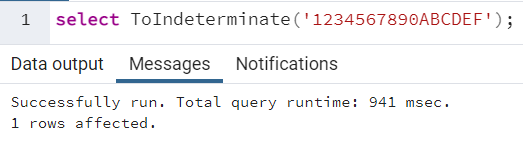
\includegraphics[width=0.8\textwidth]{Immagini/funzione1ok}
\newline\newline
Esempio di cosa accade se si prova a modificare un contratto a indeterminato se è già indeterminato.
\newline\newline
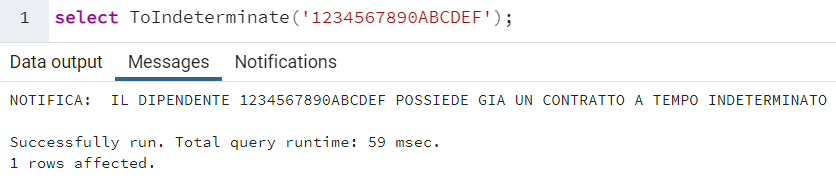
\includegraphics[width=1.1\textwidth]{Immagini/funzione1no}
\subsection{Rinnovo contratto scaduto}
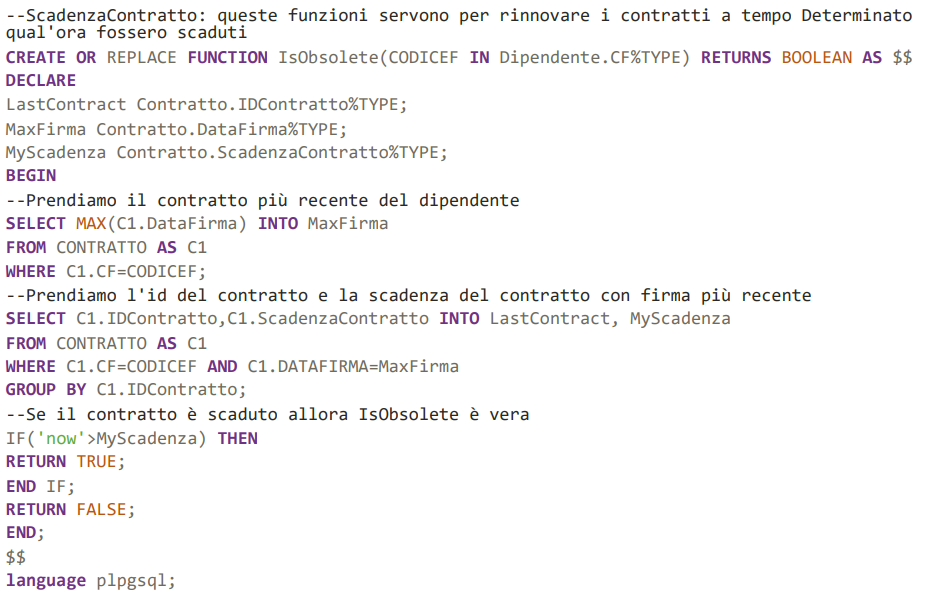
\includegraphics[width=1\textwidth]{Immagini/funzione2.sql}
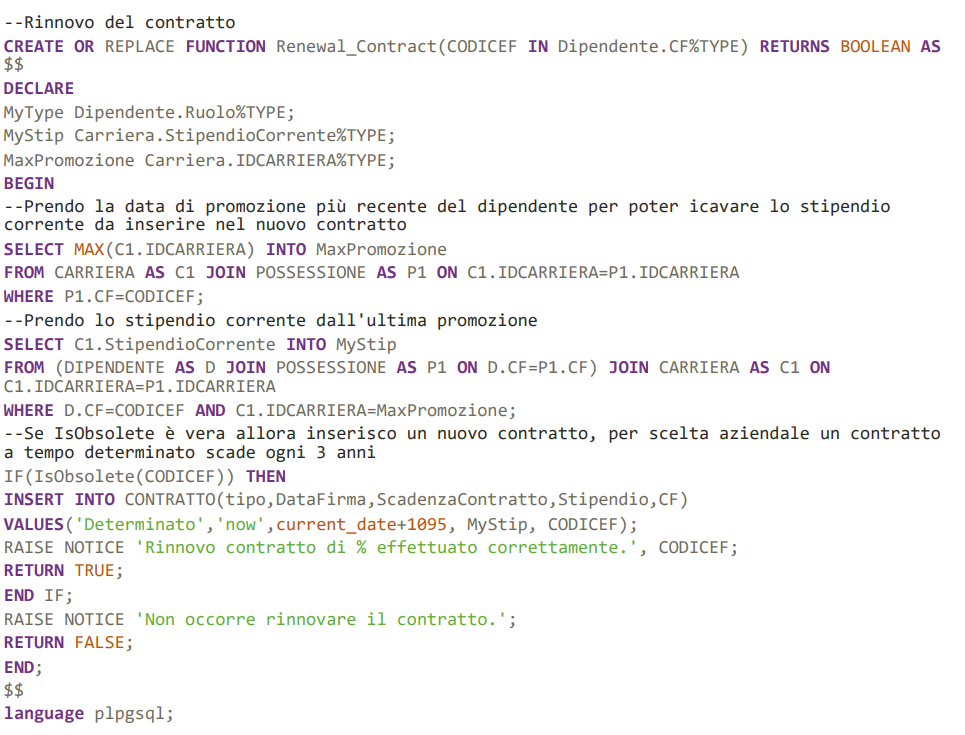
\includegraphics[width=1.1\textwidth]{Immagini/funzione2.1.sql}
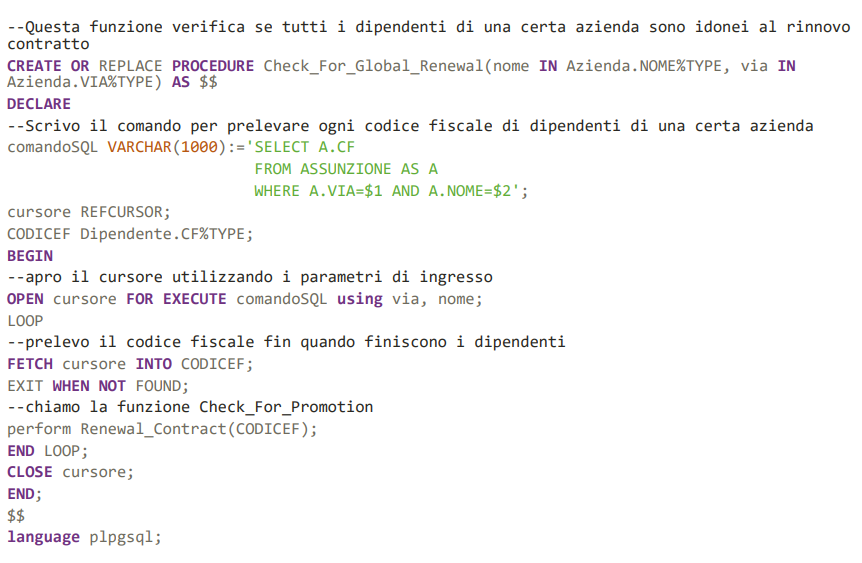
\includegraphics[width=1.1\textwidth]{Immagini/funzione2.2.sql}
\newline\newline
Esempio di cosa accade se rinnovo tutti i contratti scaduti di una certa azienda:
\newline\newline
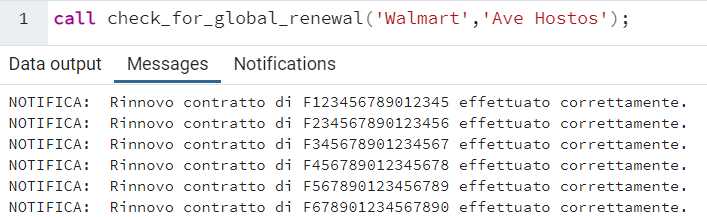
\includegraphics[width=1.1\textwidth]{Immagini/funzione2ok.png}
\subsection{Assunzione dei dipendenti e firma del contratto}
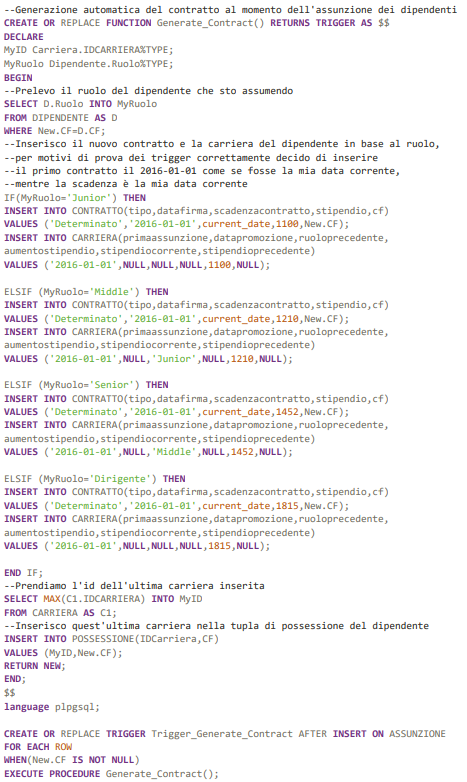
\includegraphics[width=0.9\textwidth]{Immagini/trigger1.sql}
\subsection{Utilizzo laboratori}
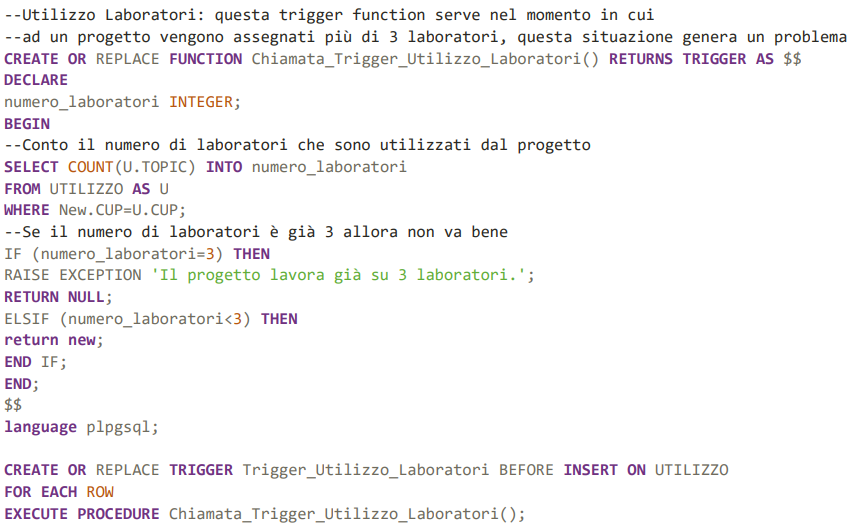
\includegraphics[width=1.1\textwidth]{Immagini/vincolo2.sql}
\newline\newline
Esempio di cosa accade se un progetto tenta di utilizzare più di 3 laboratori:
\newline\newline
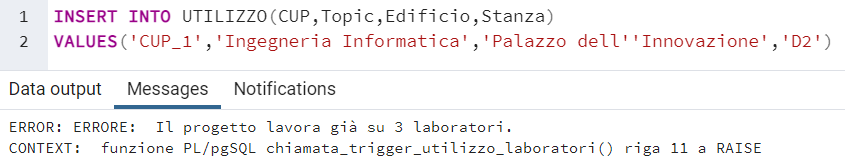
\includegraphics[width=1.1\textwidth]{Immagini/vincolo2}
\subsection{Passaggio a nuovo ruolo}
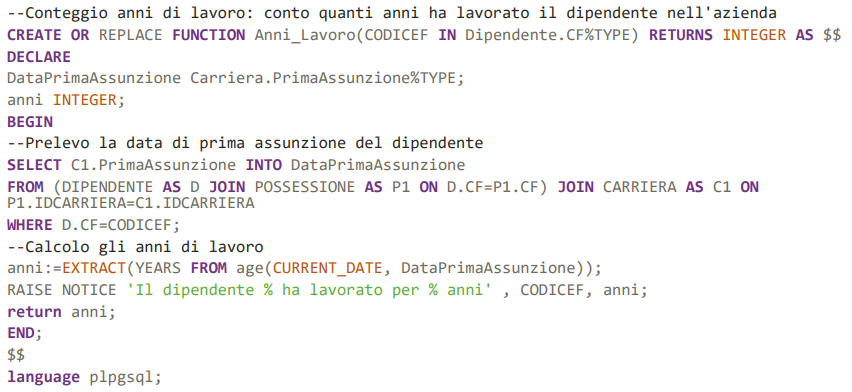
\includegraphics[width=1.1\textwidth]{Immagini/funzione3anni.sql}
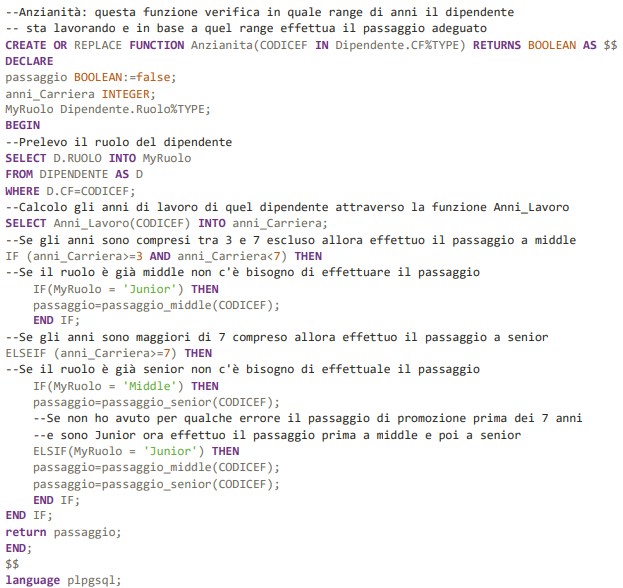
\includegraphics[width=1\textwidth]{Immagini/anzianita.sql}
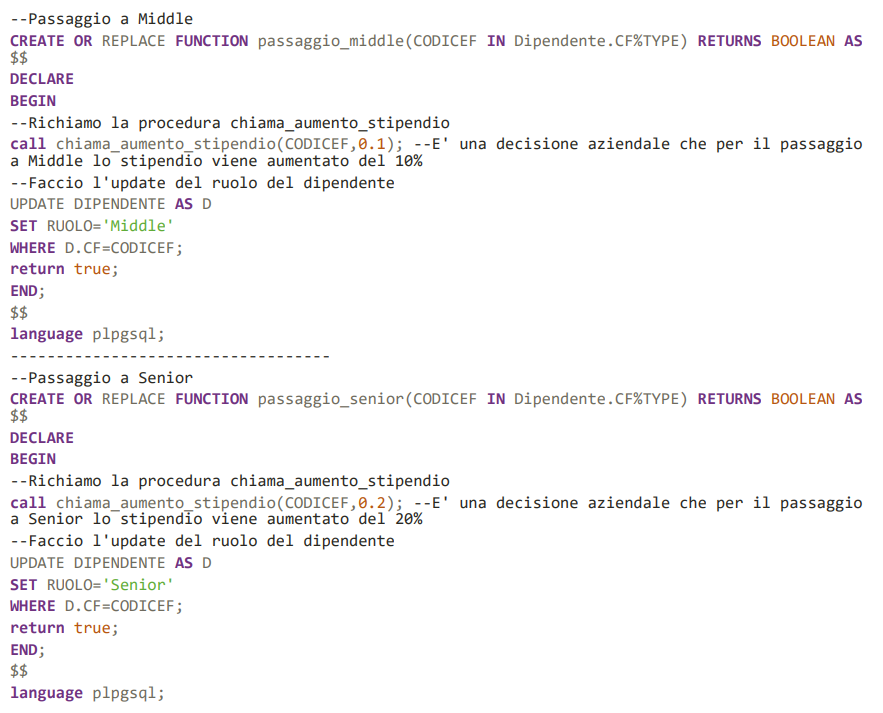
\includegraphics[width=1\textwidth]{Immagini/passaggio.sql}
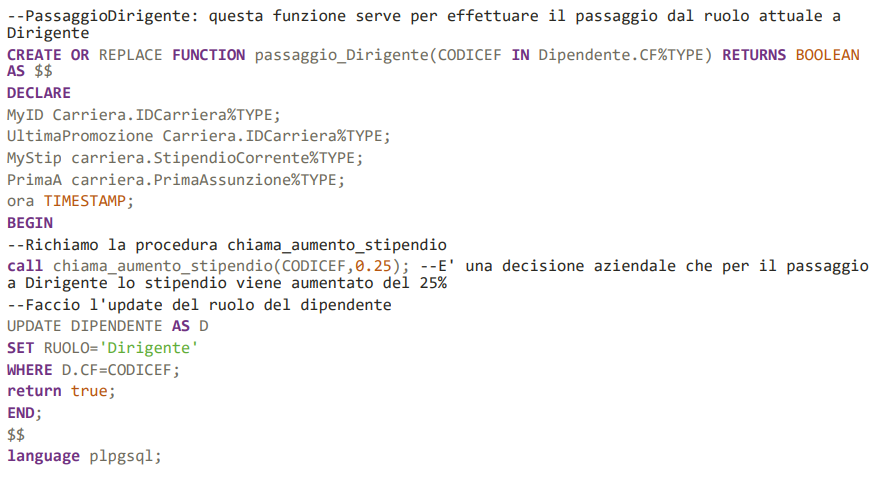
\includegraphics[width=1\textwidth]{Immagini/passaggioDir.sql}
\newpage
Esempio di cosa accade se effettuo un passaggio a Dirigente di un dipendente:
\newline\newline
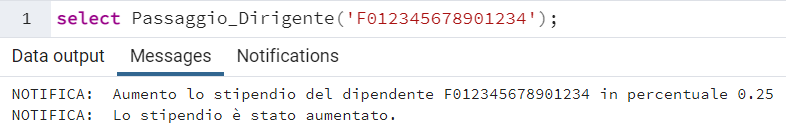
\includegraphics[width=1\textwidth]{Immagini/passaggioDir}
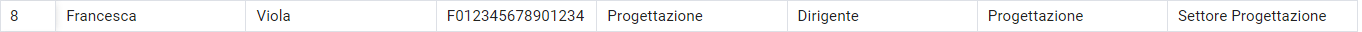
\includegraphics[width=1.2\textwidth]{Immagini/viola}
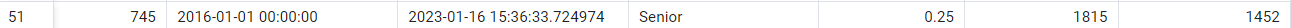
\includegraphics[width=1.2\textwidth]{Immagini/carriera}
\newline\newline
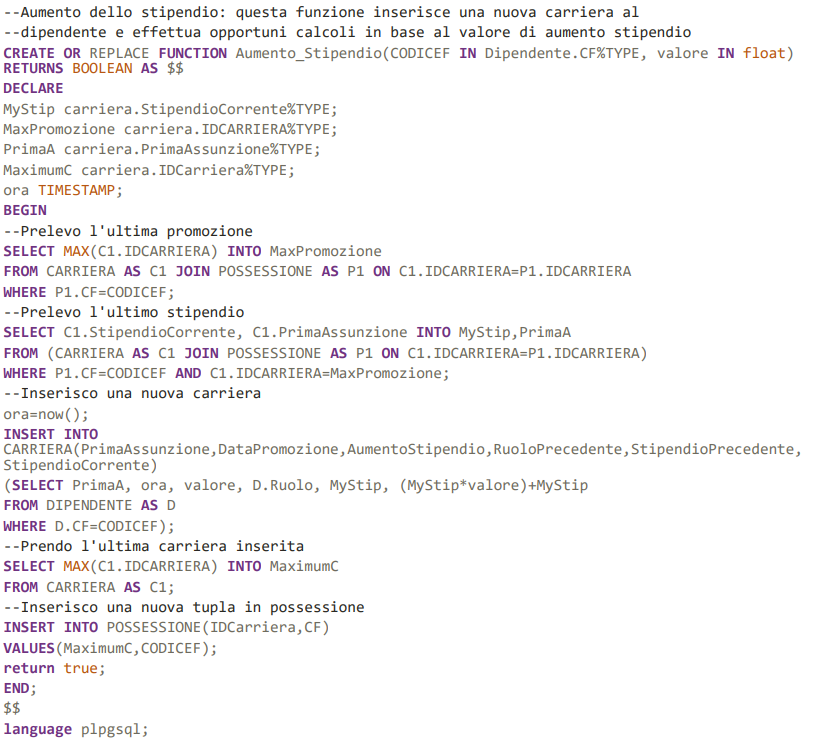
\includegraphics[width=1\textwidth]{Immagini/aumento_stip.sql}
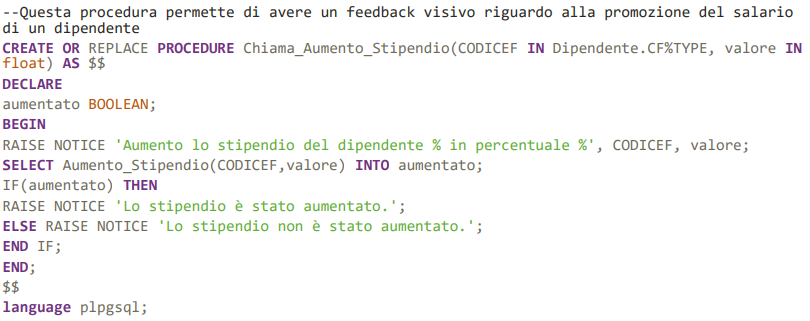
\includegraphics[width=1\textwidth]{Immagini/chiama_aum.sql.png}
Esempio di cosa accade quando aumento lo stipendio di un dipendente:
\newline\newline
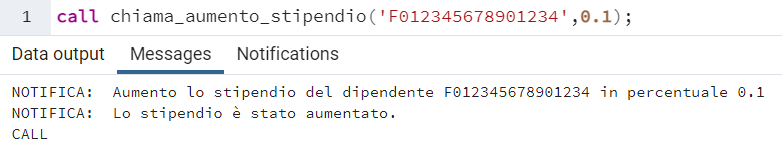
\includegraphics[width=1\textwidth]{Immagini/aum_es.png}
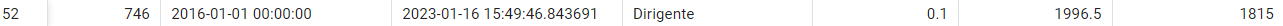
\includegraphics[width=1\textwidth]{Immagini/aum_es2.png}
\newline\newline
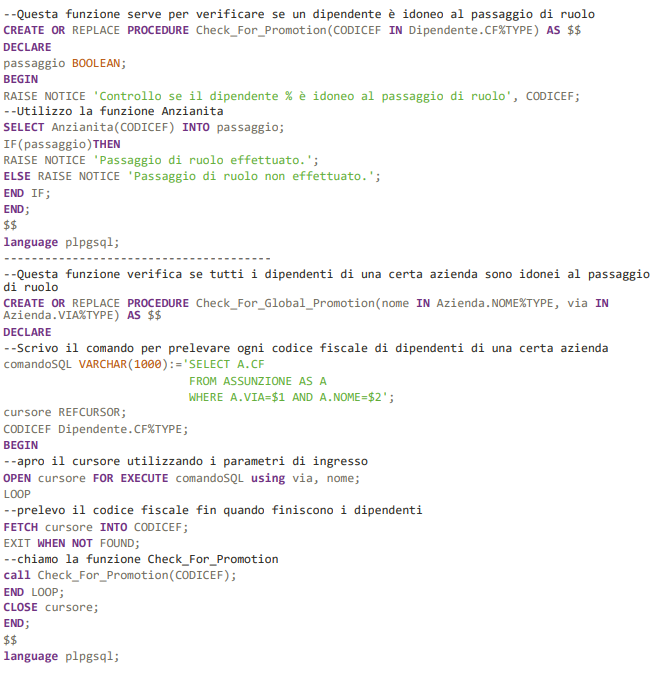
\includegraphics[width=1.2\textwidth]{Immagini/idoneopass.sql}
\newpage
Esempio di cosa accade quando verifico se i dipendenti di un'azienda
sono idonei o meno alla promozione (passaggio di ruolo):
\newline\newline
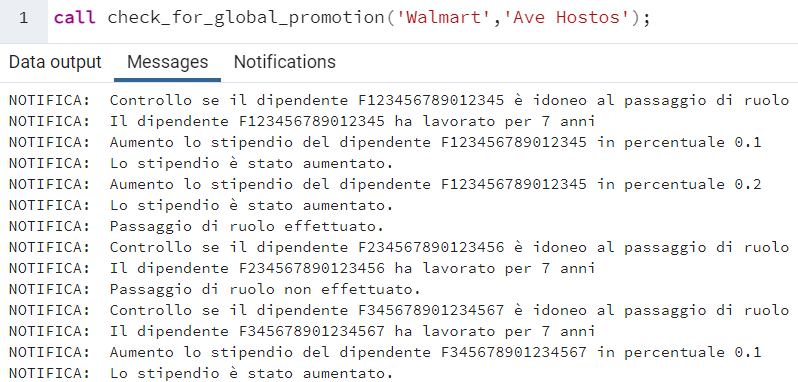
\includegraphics[width=1\textwidth]{Immagini/idonei.png}
\subsection{Consistenza data di prima assunzione}
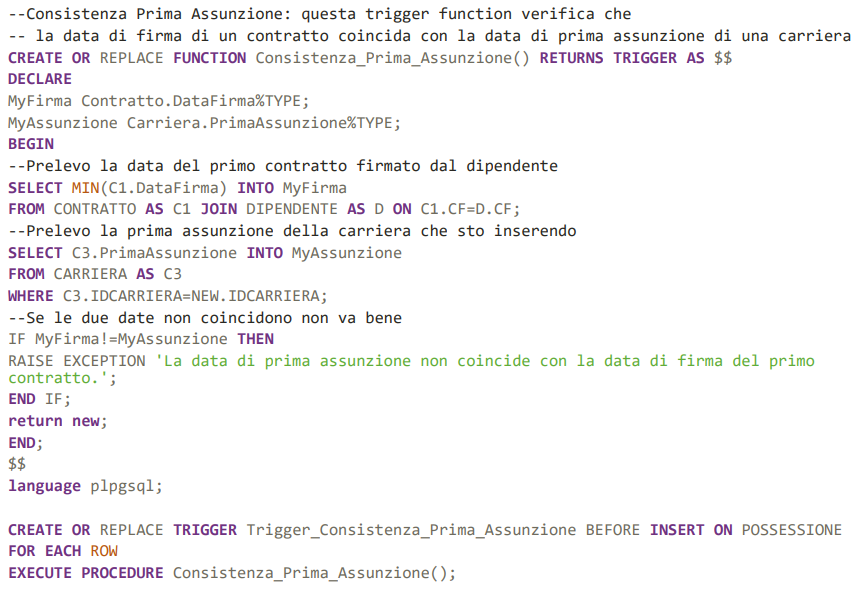
\includegraphics[width=1\textwidth]{Immagini/consistenzadate.sql}
\newpage
Esempio di cosa accade quando provo a collegare una carriera con data di prima assunzione
diversa dalla data di firma del primo contratto di un dipendente:
\newline\newline
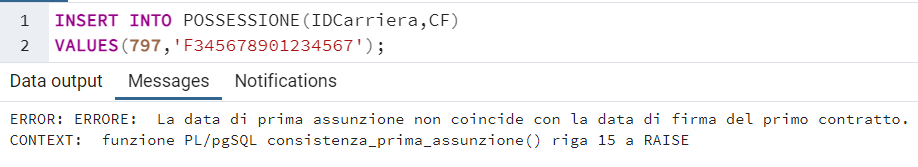
\includegraphics[width=1\textwidth]{Immagini/consdatees}
\subsection{Responsabilità progetti}
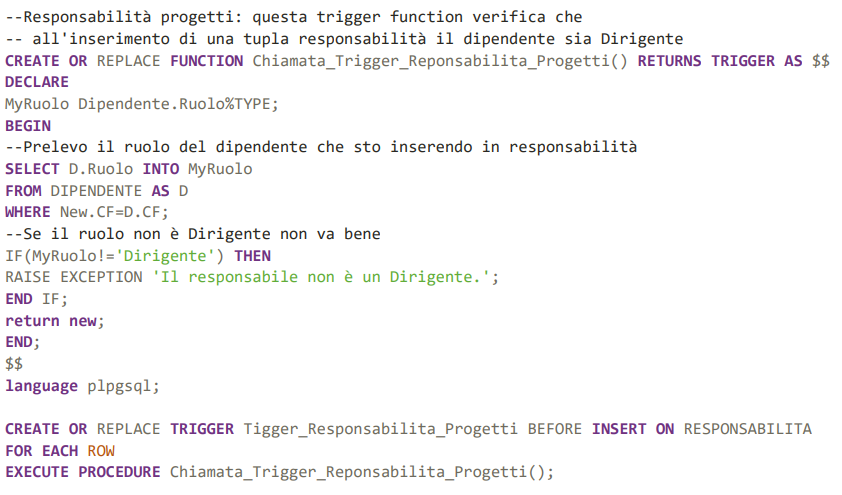
\includegraphics[width=1\textwidth]{Immagini/responsabilita.sql}
\newline\newline
Esempio di cosa accade se provo a responsabilizzare un dipendente non Dirigente:
\newline\newline
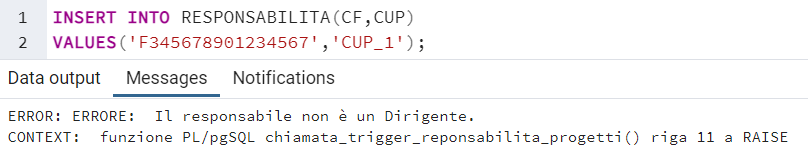
\includegraphics[width=1\textwidth]{Immagini/reses}
\subsection{Gestione Laboratori}
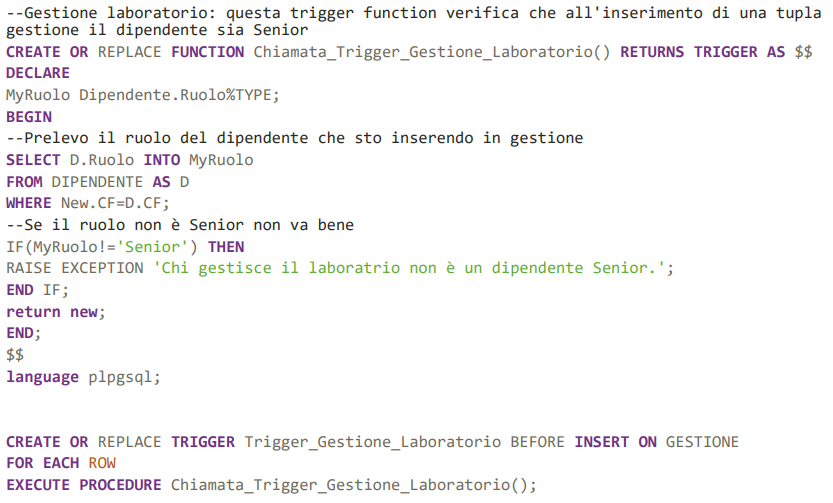
\includegraphics[width=1\textwidth]{Immagini/gestione.sql}
\newline\newline
Esempio di cosa accade se provo a far gestire un laboratorio da un dipendente non Senior:
\newline\newline
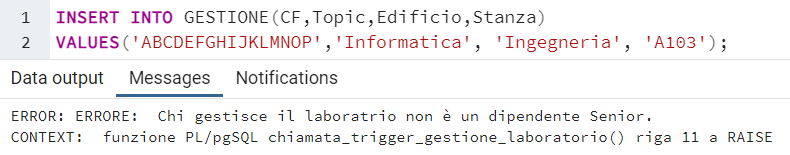
\includegraphics[width=1\textwidth]{Immagini/geses}
\subsection{Referenza Progetti}
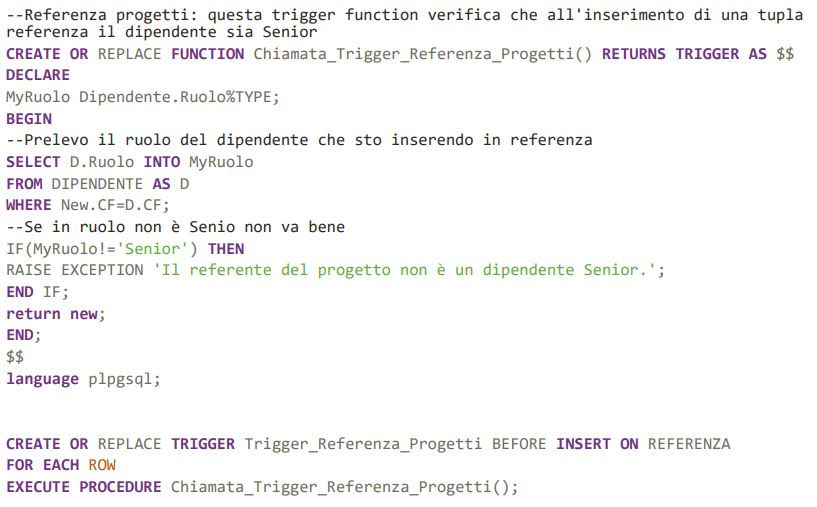
\includegraphics[width=1\textwidth]{Immagini/referenza.sql}
\newline\newline
Esempio di cosa accade se provo a far referenziare un progetto da un dipendente non Senior:
\newline\newline
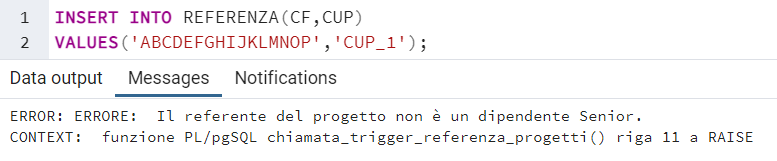
\includegraphics[width=1\textwidth]{Immagini/refes}



 

\end{document}*6